
\section{Risk analysis}
\label{section:risk_analysis}

This section will present a risk analysis for the high-level functionalities (HFL) and each of the requirements for the SoCam system. The requirements are analyzed individually and isolated, with the assumption that the related requirements are met. This is partly because of SoCam being a maintenance program, which implies that there already exist a functional system to maintain. 

The identified risks are analyzed in terms of consequence and probability, and the result of the two variables determines the severity of the risk.  Figure \ref{fig:risk_analysis} presents the scale used to determine the consequence and probability, and how the severity is determined by these two variables. \newline

\noindent Probability is divided into three levels:

\begin{enumerate}
    \item \textbf{Unlikely} - Unlikely to happen due to experienced personnel, good routines, and the available software and hardware. Almost never happens. 
    \item \textbf{Likely} - Likely to happen with even experienced personnel, good routines, and the available software and hardware. Happens occasionally.  
    \item \textbf{Very likely} - Very likely to happen with even experienced personnel, good routines, and the available software and hardware. Happens more often than not.
\end{enumerate}

\noindent Consequence is divided into three levels:

\begin{enumerate}
    \item \textbf{Minor} - Minor impact on cost in terms of money and/or time investment needed to remedy the risk. Minor impact on the involved parties. Minor impact on the rest of the system, the system flow will continue without being impeded. 
    \item \textbf{Moderate} - Moderate impact on cost in terms of money and/or time investment needed to remedy the risk. Moderate impact on the involved parties. Moderate impact on the rest of the system, the system flow will continue but may be impeded to some degree.
    \item \textbf{Major} - Major impact on cost in terms of money and/or time investment needed to remedy the risk. Major impact on the involved parties. Major impact on the rest of the system, the system flow may come to an halt.
\end{enumerate}

\begin{figure}[H]
    \centering
    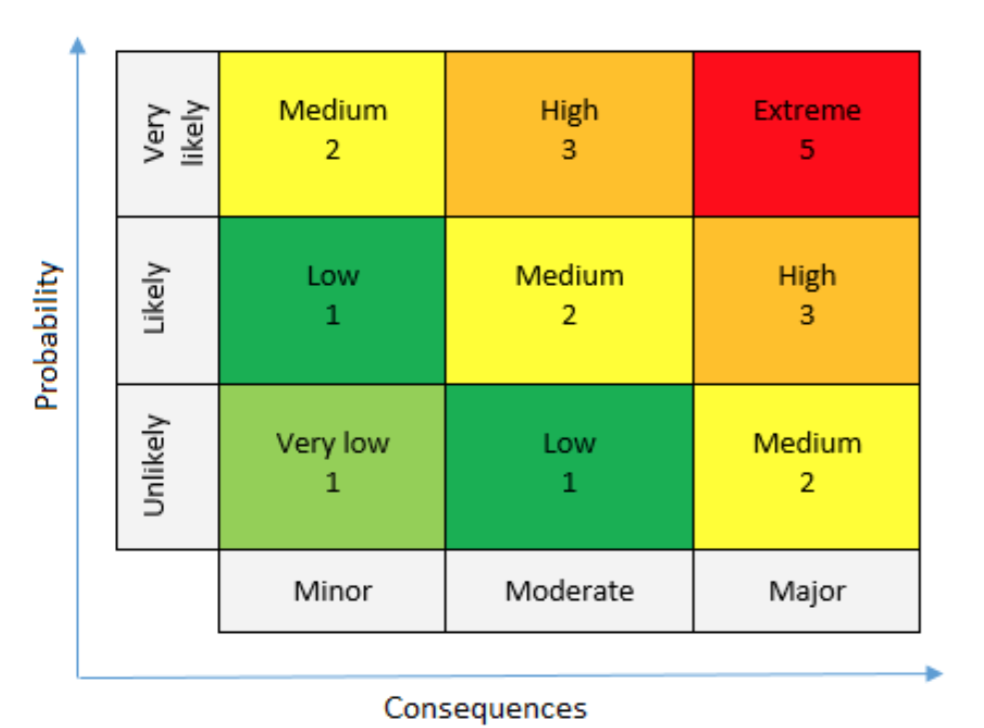
\includegraphics[scale=0.4]{images/risk_analysis}
    \caption{Risk analysis}
    \label{fig:risk_analysis}
\end{figure}

\subsection{High-level functionality}

This section will present the high-level functionalities, their risk, consequence and probability. The high-level functionalities mentioned in the exercise text was:

\begin{enumerate}
    \item Insert new software or new versions of software into a software database.
    \item Maintain a database that shows which control units need which software.
    \item Send alarm (recall) if critical defects are discovered.
    \item Assist the garage in updating car software.
\end{enumerate}

\begin{table}[H]
\centering
\caption{High-level functionality}
\label{table:hlf}
\begin{tabularx}{1.0\textwidth}{
    |p{\dimexpr.20\linewidth-2\tabcolsep-1.3333\arrayrulewidth}% column 1
    |p{\dimexpr.80\linewidth-2\tabcolsep-1.3333\arrayrulewidth}|% column 2
}
\hline

ID
& 1
\\
\hline

HFL
& Insert new software and new versions of existing software into a software database
\\
\hline

Risk
& 
The inserted software is erroneous
\\
\hline

Consequence
&
Moderate
\\
\hline

Probability
&
Likely
\\
\hline

Total risk
&
Medium
\\
\hline


\end{tabularx}
\end{table}

% ---------------- %
% ---------------- %

\begin{table}[H]
\centering
\begin{tabularx}{1.0\textwidth}{
    |p{\dimexpr.20\linewidth-2\tabcolsep-1.3333\arrayrulewidth}% column 1
    |p{\dimexpr.80\linewidth-2\tabcolsep-1.3333\arrayrulewidth}|% column 2
}
\hline

ID
& 2
\\
\hline

HFL
& Maintain a database that shows which control units (ECU) that needs which software
\\
\hline

Risk
& 
The ECUs are mapped to wrong software
\\
\hline

Consequence
&
Major
\\
\hline

Probability
&
Likely
\\
\hline

Total risk
&
High
\\
\hline

\end{tabularx}
\end{table}

% ---------------- %
% ---------------- %

\begin{table}[H]
\centering
\begin{tabularx}{1.0\textwidth}{
    |p{\dimexpr.20\linewidth-2\tabcolsep-1.3333\arrayrulewidth}% column 1
    |p{\dimexpr.80\linewidth-2\tabcolsep-1.3333\arrayrulewidth}|% column 2
}
\hline

ID
& 3
\\
\hline

HFL
& Send an alarm (”recall”) if we discover critical defects
\\
\hline

Risks
& 
The alarm is not sent when critical defects are discovered
\\
\hline

Consequence
&
Major
\\
\hline

Probability
&
Unlikely
\\
\hline

Total risk
&
Medium
\\
\hline

\end{tabularx}
\end{table}

% ---------------- %
% ---------------- %

\begin{table}[H]
\centering
\begin{tabularx}{1.0\textwidth}{
    |p{\dimexpr.20\linewidth-2\tabcolsep-1.3333\arrayrulewidth}% column 1
    |p{\dimexpr.80\linewidth-2\tabcolsep-1.3333\arrayrulewidth}|% column 2
}
\hline

ID
& 4
\\
\hline

HFL
& Assist the garage in updating care software
\\
\hline

Risk
& 
SoCam is unable to assist the garage in updating the car software
\\
\hline

Consequence
&
Moderate
\\
\hline

Probability
&
Unlikely
\\
\hline

Total risk
&
Low
\\
\hline

\end{tabularx}
\end{table}

\subsection{Requirements specification}
\label{section:requirements_specification}

This section will go in-depth into each of the requirements of the SoCam system. 

\subsubsection{Manufacturer system}

This section will present the requirements, their risk, probability, and consequence of the manufacturer system. 

\begin{table}[H]
\centering
\caption{Manufacturer system requirements}
\label{table:manufacturer}
\begin{tabularx}{1.0\textwidth}{
    |p{\dimexpr.20\linewidth-2\tabcolsep-1.3333\arrayrulewidth}% column 1
    |p{\dimexpr.80\linewidth-2\tabcolsep-1.3333\arrayrulewidth}|% column 2
}
\hline

Req. ID
& 1.1
\\
\hline

Requirement
& The new software and new versions of software the CM enters shall be stored in a software archive
\\
\hline

Risk
& 
The software entered by the CM into the software archive can be erroneous.
\\
\hline

Consequence
&
Moderate
\\
\hline

Probability
&
Likely
\\
\hline

Total risk
&
Medium
\\
\hline

\end{tabularx}
\end{table}

% ---------------- %
% ---------------- %

\begin{table}[H]
\centering
\begin{tabularx}{1.0\textwidth}{
    |p{\dimexpr.20\linewidth-2\tabcolsep-1.3333\arrayrulewidth}% column 1
    |p{\dimexpr.80\linewidth-2\tabcolsep-1.3333\arrayrulewidth}|% column 2
}
\hline
Req. ID
& 1.2
\\
\hline

Requirement
& The software shall version the software components by subnumbering the unique part number
\\
\hline

Risk
& 
The software entered into the software archive does not receive the correct subnumber for versioning
\\
\hline

Consequence
&
Moderate
\\
\hline

Probability
&
Unlikely
\\
\hline

Total risk
&
Low
\\
\hline

\end{tabularx}
\end{table}

% ---------------- %
% ---------------- %

\begin{table}[H]
\centering
\begin{tabularx}{1.0\textwidth}{
    |p{\dimexpr.20\linewidth-2\tabcolsep-1.3333\arrayrulewidth}% column 1
    |p{\dimexpr.80\linewidth-2\tabcolsep-1.3333\arrayrulewidth}|% column 2
}
\hline
Req. ID
& 1.3
\\
\hline

Requirement
& The action scripts the CM enters shall be inserted in the action database
\\
\hline

Risk
& 
The action script the CM enters can be faulty
\\
\hline

Consequence
&
Moderate
\\
\hline

Probability
&
Likely
\\
\hline

Total risk
&
Medium
\\
\hline

\end{tabularx}
\end{table}

% ---------------- %
% ---------------- %

\begin{table}[H]
\centering
\begin{tabularx}{1.0\textwidth}{
    |p{\dimexpr.20\linewidth-2\tabcolsep-1.3333\arrayrulewidth}% column 1
    |p{\dimexpr.80\linewidth-2\tabcolsep-1.3333\arrayrulewidth}|% column 2
}
\hline
Req. ID
& 1.4
\\
\hline

Requirement
& The action scripts shall be updatable by the CM
\\
\hline

Risk
& 
The updated action script can be faulty
\\
\hline

Consequence
&
Moderate
\\
\hline

Probability
&
Likely
\\
\hline

Total risk
&
Medium
\\
\hline

\end{tabularx}
\end{table}

% ---------------- %
% ---------------- %

\begin{table}[H]
\centering
\begin{tabularx}{1.0\textwidth}{
    |p{\dimexpr.20\linewidth-2\tabcolsep-1.3333\arrayrulewidth}% column 1
    |p{\dimexpr.80\linewidth-2\tabcolsep-1.3333\arrayrulewidth}|% column 2
}
\hline
Req. ID
& 1.5
\\
\hline

Requirement
& The action script shall give information of which ECU needs which software component.
\\
\hline

Risk
& 
The action script gives the wrong information on which ECU needs which software component
\\
\hline

Consequence
&
Major
\\
\hline

Probability
& 
Unlikely
\\
\hline

Total risk
&
Medium
\\
\hline

\end{tabularx}
\end{table}

% ---------------- %
% ---------------- %

\begin{table}[H]
\centering
\begin{tabularx}{1.0\textwidth}{
    |p{\dimexpr.20\linewidth-2\tabcolsep-1.3333\arrayrulewidth}% column 1
    |p{\dimexpr.80\linewidth-2\tabcolsep-1.3333\arrayrulewidth}|% column 2
}
\hline
Req. ID
& 1.6
\\
\hline

Requirement
& The action script shall connect the ECU to the software component that is used to control it
\\
\hline

Risk
& 
The action script connects the ECU to the wrong software component
\\
\hline

Consequence
&
Major
\\
\hline

Probability
&
Unlikely
\\
\hline

Total risk
&
Medium
\\
\hline

\end{tabularx}
\end{table}

% ---------------- %
% ---------------- %


\begin{table}[H]
\centering
\begin{tabularx}{1.0\textwidth}{
    |p{\dimexpr.20\linewidth-2\tabcolsep-1.3333\arrayrulewidth}% column 1
    |p{\dimexpr.80\linewidth-2\tabcolsep-1.3333\arrayrulewidth}|% column 2
}
\hline
Req. ID
& 1.7
\\
\hline

Requirement
& The entry for a new production series defined by the CM shall be inserted into the vehicle database
\\
\hline

Risk
& 
The vehicle database entry may contain wrong information
\\
\hline

Consequence
& 
Major
\\
\hline

Probability
&
likely   
\\
\hline

Total risk
&
High
\\
\hline

\end{tabularx}
\end{table}

% ---------------- %
% ---------------- %

\begin{table}[H]
\centering
\begin{tabularx}{1.0\textwidth}{
    |p{\dimexpr.20\linewidth-2\tabcolsep-1.3333\arrayrulewidth}% column 1
    |p{\dimexpr.80\linewidth-2\tabcolsep-1.3333\arrayrulewidth}|% column 2
}
\hline
Req. ID
& 1.8
\\
\hline

Requirement
& Through the system the CM shall be able to identify all the vehicles with faulty components
\\
\hline

Risk
& 
The faulty component of one or more vehicles is not identified
\\
\hline

Consequence
& 
Major
\\
\hline

Probability
&
Likely
\\
\hline

Total risk
&
High
\\
\hline

\end{tabularx}
\end{table}

% ---------------- %
% ---------------- %

\begin{table}[H]
\centering
\begin{tabularx}{1.0\textwidth}{
    |p{\dimexpr.20\linewidth-2\tabcolsep-1.3333\arrayrulewidth}% column 1
    |p{\dimexpr.80\linewidth-2\tabcolsep-1.3333\arrayrulewidth}|% column 2
}
\hline
Req. ID
& 1.9
\\
\hline

Requirement
& The CM shall be able to send information plus the new version of all components to all registered garages
\\
\hline

Risk
& 
Data is not sent to all registered garages 
\\
\hline

Consequence
&
Moderate
\\
\hline

Probability
&
Likely
\\
\hline

Total risk
&
Medium
\\
\hline

\end{tabularx}
\end{table}

%
%
%
%
%
%
%
%
%
%
%

\subsubsection{Garage system}

This section will present the requirements, their risk, probability, and consequence of the garage system. 

\begin{table}[H]
\centering
\caption{Garage system requirements}
\label{table:garage}
\begin{tabularx}{1.0\textwidth}{
    |p{\dimexpr.20\linewidth-2\tabcolsep-1.3333\arrayrulewidth}% column 1
    |p{\dimexpr.80\linewidth-2\tabcolsep-1.3333\arrayrulewidth}|% column 2
}
\hline

Req. ID
& 2.1
\\
\hline

Requirement
& The system has the customer information and the vehicle's serial number for each sold vehicle in a customer database
\\
\hline

Risk
& 
The system has the wrong information
\\
\hline

Consequence
&
Moderate
\\
\hline

Probability
&
Likely
\\
\hline

Total risk
&
Medium
\\
\hline

\end{tabularx}
\end{table}

% ---------------- %
% ---------------- %

\begin{table}[H]
\centering
\begin{tabularx}{1.0\textwidth}{
    |p{\dimexpr.20\linewidth-2\tabcolsep-1.3333\arrayrulewidth}% column 1
    |p{\dimexpr.80\linewidth-2\tabcolsep-1.3333\arrayrulewidth}|% column 2
}
\hline

Req. ID
& 2.2
\\
\hline

Requirement
& The system shall download the vehicle's configuration information from the vehicle's main computer and the vehicle database by using the vehicle's serial number as a key
\\
\hline

Risk
& 
The wrong serial number key is used to obtain information or the vehicle's configuration information is erroneous
\\
\hline

Consequence
&
Moderate
\\
\hline

Probability
&
Unlikely
\\
\hline

Total risk
&
Low
\\
\hline

\end{tabularx}
\end{table}

% ---------------- %
% ---------------- %

\begin{table}[H]
\centering
\begin{tabularx}{1.0\textwidth}{
    |p{\dimexpr.20\linewidth-2\tabcolsep-1.3333\arrayrulewidth}% column 1
    |p{\dimexpr.80\linewidth-2\tabcolsep-1.3333\arrayrulewidth}|% column 2
}
\hline

Req. ID
& 2.3
\\
\hline

Requirement
& The system shall use the two sets of configuration information to identify the latest version of each software component for each ECU in the vehicle
\\
\hline

Risk
& 
Software version for one or more component cannot be identified or differs from the last version
\\
\hline

Consequence
&
Moderate
\\
\hline

Probability
&
Unlikely
\\
\hline

Total risk
&
Low
\\
\hline

\end{tabularx}
\end{table}

% ---------------- %
% ---------------- %

\begin{table}[H]
\centering
\begin{tabularx}{1.0\textwidth}{
    |p{\dimexpr.20\linewidth-2\tabcolsep-1.3333\arrayrulewidth}% column 1
    |p{\dimexpr.80\linewidth-2\tabcolsep-1.3333\arrayrulewidth}|% column 2
}
\hline

Req. ID
& 2.4
\\
\hline

Requirement
& The system shall download the latest version of all components that are needed for the vehicle but not yet installed 
\\
\hline

Risk
& 
The system downloads and installs the wrong software version
\\
\hline

Consequence
&
Major
\\
\hline

Probability
&
Unlikely
\\
\hline

Total risk
&
Medium
\\
\hline

\end{tabularx}
\end{table}

% ---------------- %
% ---------------- %

\begin{table}[H]
\centering
\begin{tabularx}{1.0\textwidth}{
    |p{\dimexpr.20\linewidth-2\tabcolsep-1.3333\arrayrulewidth}% column 1
    |p{\dimexpr.80\linewidth-2\tabcolsep-1.3333\arrayrulewidth}|% column 2
}
\hline

Req. ID
& 2.5
\\
\hline

Requirement
& The system shall install all new software components
\\
\hline

Risk
& 
One or more software component installations fails
\\
\hline

Consequence
&
Minor
\\
\hline

Probability
&
Likely
\\
\hline

Total risk
&
Low
\\
\hline

\end{tabularx}
\end{table}

% ---------------- %
% ---------------- %

\begin{table}[H]
\centering
\begin{tabularx}{1.0\textwidth}{
    |p{\dimexpr.20\linewidth-2\tabcolsep-1.3333\arrayrulewidth}% column 1
    |p{\dimexpr.80\linewidth-2\tabcolsep-1.3333\arrayrulewidth}|% column 2
}
\hline

Req. ID
& 2.6
\\
\hline

Requirement
& The system shall update the history log and send it to the action database
\\
\hline

Risk
& 
The updated history log is erroneous
\\
\hline

Consequence
&
Moderate
\\
\hline

Probability
&
Likely
\\
\hline

Total risk
&
Medium
\\
\hline

\end{tabularx}
\end{table}

% ---------------- %
% ---------------- %

\begin{table}[H]
\centering
\begin{tabularx}{1.0\textwidth}{
    |p{\dimexpr.20\linewidth-2\tabcolsep-1.3333\arrayrulewidth}% column 1
    |p{\dimexpr.80\linewidth-2\tabcolsep-1.3333\arrayrulewidth}|% column 2
}
\hline

Req. ID
& 2.7
\\
\hline

Requirement
& The system shall update the vehicle's configuration information
\\
\hline

Risk
& 
The updated vehicle's configuration information is faulty or the vehicle's configuration information is not updated
\\
\hline

Consequence
&
Moderate
\\
\hline

Probability
&
Likely
\\
\hline

Total risk
&
Medium
\\
\hline

\end{tabularx}
\end{table}

% ---------------- %
% ---------------- %

\begin{table}[H]
\centering
\begin{tabularx}{1.0\textwidth}{
    |p{\dimexpr.20\linewidth-2\tabcolsep-1.3333\arrayrulewidth}% column 1
    |p{\dimexpr.80\linewidth-2\tabcolsep-1.3333\arrayrulewidth}|% column 2
}
\hline

Req. ID
& 2.8
\\
\hline

Requirement
& The system shall updated vehicle's configuration information in the vehicle database 
\\
\hline

Risk
& 
The vehicle database is updated with faulty vehicle configuration information or not updated with the vehicle configuration information
\\
\hline

Consequence
&
Moderate
\\
\hline

Probability
&
Likely
\\
\hline

Total risk
&
Medium
\\
\hline

\end{tabularx}
\end{table}

% ---------------- %
% ---------------- %

\begin{table}[H]
\centering
\begin{tabularx}{1.0\textwidth}{
    |p{\dimexpr.20\linewidth-2\tabcolsep-1.3333\arrayrulewidth}% column 1
    |p{\dimexpr.80\linewidth-2\tabcolsep-1.3333\arrayrulewidth}|% column 2
}
\hline

Req. ID
& 2.9
\\
\hline

Requirement
& The system shall use the customer database to identify the vehicle's serial number based on customer name and vice versa
\\
\hline

Risk
& 
The vehicle's serial number is mapped  to the wrong customer name
\\
\hline

Consequence
&
Moderate
\\
\hline

Probability
&
Likely

\\
\hline

Total risk
&
Medium 
\\
\hline

\end{tabularx}
\end{table}

